\documentclass[a4paper,12pt]{article}
\setlength{\parindent}{0cm}
\usepackage{amsmath, amssymb, amsthm, mathtools,pgfplots}
\usepackage{graphicx,caption}
\usepackage{verbatim}
\usepackage{venndiagram}
\usepackage[cm]{fullpage}
\usepackage{fancyhdr}
\usepackage{tikz,multirow}
\usepackage{listings}
\usepackage{color,enumerate,framed}
\usepackage{color,hyperref}
\definecolor{darkblue}{rgb}{0.0,0.0,0.5}
\hypersetup{colorlinks,breaklinks,
            linkcolor=darkblue,urlcolor=darkblue,
            anchorcolor=darkblue,citecolor=darkblue}

%\usepackage{tgadventor}
%\usepackage[nohug]{diagrams}
\usepackage[T1]{fontenc}
%\usepackage{helvet}
%\renewcommand{\familydefault}{\sfdefault}
%\usepackage{parskip}
%\usepackage{picins} %for \parpic.
%\newtheorem*{notation}{Notation}
%\newtheorem{example}{Example}[section]
%\newtheorem*{problem}{Problem}
\theoremstyle{definition}
%\newtheorem{theorem}{Theorem}
%\newtheorem*{solution}{Solution}
%\newtheorem*{definition}{Definition}
%\newtheorem{lemma}[theorem]{Lemma}
%\newtheorem{corollary}[theorem]{Corollary}
%\newtheorem{proposition}[theorem]{Proposition}
%\newtheorem*{remark}{Remark}
%\setcounter{section}{1}

\newtheorem{thm}{Theorem}[section]
\newtheorem{lemma}[thm]{Lemma}
\newtheorem{prop}[thm]{Proposition}
\newtheorem{cor}[thm]{Corollary}
%\newtheorem{defn}[thm]{Definition}
\newtheorem*{defn}{Definition}
\newtheorem*{examp}{Example}
\newtheorem{conj}[thm]{Conjecture}
\newtheorem{rmk}[thm]{Remark}
\newtheorem*{nte}{Note}
\newtheorem*{notat}{Notation}
%\pgfplotset{compat=1.14}
%\diagramstyle[labelstyle=\scriptstyle]

\lstset{frame=tb,
  language=Oz,
  aboveskip=3mm,
  belowskip=3mm,
  showstringspaces=false,
  columns=flexible,
  basicstyle={\small\ttfamily},
  breaklines=true,
  breakatwhitespace=true,
  tabsize=3
}

\usepackage{floatrow}
% Table float box with bottom caption, box width adjusted to content
\newfloatcommand{capbtabbox}{table}[][\FBwidth]

\pagestyle{fancy}




\fancyhead{}
\renewcommand{\headrulewidth}{0pt}

\lfoot{}
\cfoot{}

%\lfoot{\color{black!60}{\sffamily Zhangsheng Lai}}
\cfoot{\color{black!60}{\sffamily Last modified: \today}}
\rfoot{\textsc{\thepage}}



\begin{document}
\flushright{Nguyen Tan Thai Hung\quad *number*\\Zhangsheng Lai\quad1002554}
\section*{Algorithmic Game Theory: HW 1}

\begin{enumerate}
\item To show the desired inequality, it suffices to show that $f(y,z) = 5y^2+z^2-3zy-3y \geq 0$ for every $y, z \in \{0,1,2,\ldots\}$. We shall use $\mathbb{Z}_{>0}$ to denote the set $\{0,1,2,\ldots\}$ subsequently. We can rewrite $f(y,z)$ to get
\begin{align}
f(y,z) = \left(\frac{3}{2}y-z\right)^2+\frac{11}{4}y^2-3y \label{eq:pos}
\end{align}
which we will show that the $f(y,z)$ in this form is nonnegative. All that is left to show is that  $\frac{11}{4}y^2-3y \geq 0$ for all $y\in \mathbb{Z}_{>0}$ but solving for the inequality, we have
\begin{align*}
\frac{11}{4}y^2-3y \geq 0 \Leftrightarrow y \geq \frac{12}{11} \text{ or } y=0
\end{align*}
meaning we are left to prove that (\ref{eq:pos}) holds for all $z \in \mathbb{Z}_{>0}$ when $y=1$. Solving for the inequality below, 
\begin{align*}
f(1,z)=\left(z-\frac{3}{2}\right)^2-\frac{1}{4} < 0 &\Leftrightarrow (z-1)(z-2)< 0\\
&\Leftrightarrow 1<z<2
\end{align*} 
which says that $f(1,z)<0$ for $z \in (1,2)$ and hence positive for all $z \in \mathbb{Z}_{>0}$ and we are done.

\item 
\begin{enumerate}[(i)]
\item In an nonatomic congestion games with multicommodity networks, let $\mathcal{P}_i$ denote the set of paths from an origin $s_i$ to a sink $t_i$ with $\mathcal{P}_i\neq \emptyset$.
\begin{defn}[flow]
For a \emph{flow} $f$ and path $P \in \mathcal{P}_i$, $f_P$ is the amount of traffic of commodity $i$ that chooses the path $P$ to travel from $s_i$ to $t_i$. A flow is feasible for a vector $r=(r_1,\ldots,r_k)$ if it routes all the traffic: for each $i\in \{1, 2, \ldots, k\}$, $\sum_{P\in \mathcal{P}_i}f_P=r_i$.
\end{defn}
\begin{defn}[Nonatomic equilibrium flow]
Let $f$ be a feasible flow for an nonatomic congestion games with multicommodity networks. The flow $f$ is an \emph{equilibrium flow} if, for every commodity $i \in \{1,2, \ldots, k\}$ and every pair $P, \tilde{P} \in \mathcal{P}_i$ of $s_i-t_i$ paths with $f_P>0$, 
\begin{align*}
c_p(f) \leq c_{\tilde{P}}(f)
\end{align*}
where $c_p(f)$ denotes the cost of travelling on path $P$ for flow $f$.
\end{defn}
\item Let $\mathcal{P}=\bigcup_{i=1}^{k}\mathcal{P}_i$. Then the total cost of a multicommodity network is 
\begin{align*}
\sum_{P\in \mathcal{P}}c_p(f_p)\cdot f_p = \sum_{e\in E}c_e(f_e)\cdot f_e
\end{align*}
where $E$ is the set of directed edges on the graph $G$.
\item
\item We start by showing that 
\begin{align*}
\inf_{x}\left\{\left(\frac{ax+b}{ar+b}-1\right)\right\}&=\inf_{x}\left\{x\left(\frac{a(x-r)}{ar+b}\right)\right\}\\
&=\frac{a}{ar+b}\inf_{x}\left\{x^2-rx\right\}\\
&=-\frac{r^2}{4}\cdot\frac{a}{ar+b}\\
\end{align*}
with that we can begin out proof.
\begin{align*}
\sup_{c\in \mathcal{C}}\sup_{x,r}\frac{rc(r)}{x c(x)-(r-x)c(r)}&=\sup_{c\in \mathcal{C}}\sup_{x,r}\frac{r}{r +x\left(\frac{c(x)}{c(r)}-1\right)}, \text{ since $c(r)>0$}
\\
&=\sup_{a,b\geq0}\sup_{x,r}\frac{r}{r +x\left(\frac{ax+b}{ar+b}-1\right)}\\
&=\sup_{a,b\geq0}\sup_{r}\frac{r}{r -\frac{r^2}{4}\frac{a}{ar+b}}\\
&=\sup_{a,b\geq0}\sup_{r}\frac{1}{1 -\frac{ar}{4(ar+b)}}\\
&=\frac{1}{1-1/4}
\end{align*}
the last equality follows as the supremum of $\frac{ar}{4(ar+b)}$ occurs when $b=0$.
\end{enumerate}

\item
\begin{enumerate}[(i)]
\item Let $\Phi$ be the potential function of a potential game and $c_i$ denote the cost function of the agents for $i\in \{1,2,\ldots,k\}$. 
%If $s=(s_1,\ldots,s_{i-1},s_i,s_{i+1},\ldots,s_k)$ and $s'_i \neq s_i$ is any alternative strategy for agent $i$ for $i\in \{1,2,\ldots,k\}$, we have
%\begin{align*}
%c_i(s_i,s_{-i})-c_i(s'_i,s_{-i})=\Phi(s_i,s_{-i})-\Phi(s'_i,s_{-i})
%\end{align*}
To prove the required, it suffices to show that 
\begin{align*}
c_i(s_i,s_{-i})-\Phi(s_i,s_{-i})
\end{align*}
is independent of the choice of $s_i$ and solely dependent on $s_{-i}$. If we consider two alternative distinct strategies for agent $i$, $s'_i, s''_i \neq s_i$
\begin{align*}
c_i(s_i,s_{-i})&=\Phi(s_i,s_{-i})+\left[c_i(s'_i,s_{-i})-\Phi(s'_i,s_{-i})\right]\\
c_i(s_i,s_{-i})&=\Phi(s_i,s_{-i})+\left[c_i(s''_i,s_{-i})-\Phi(s''_i,s_{-i})\right]
\end{align*} 
hence we can choose $D_i(s_{-i})=c_i(-,s_{-i})-\Phi(-,s_{-i})$, where $-$ represents any choice of strategy of agent $i$.

\item Let $\Phi_1$ and $\Phi_2$ be two potential functions of a game. From 3\,(i) we have
\begin{align}
c_i(s_i,s_{-i})&=\Phi_1(s_i,s_{-i})+D^1_i(s_{-i})\label{eq:3ii1}\\
c_i(s_i,s_{-i})&=\Phi_2(s_i,s_{-i})+D^2_i(s_{-i})\label{eq:3ii2}
\end{align}
where $D^k_i(s_{-i})$ denotes the dummy term for $k=1,2$. Taking (\ref{eq:3ii1})$-$(\ref{eq:3ii2}), 
 \begin{align*}
\Phi_1(s_i,s_{-i})-\Phi_2(s_i,s_{-i})=D^1_i(s_{-i})-D^2_i(s_{-i})
\end{align*}
we have shown that two distinct potential functions differ by a constant, more precisely the difference of their dummy term evaluated at $s_{-i}$ and any strategy of agent $i$, $s_i$.

\item
$(\Rightarrow)$: Let $\Phi$ be a potential function for a finite game. We want to show:
\begin{align*}
c_i(s^2_i,s^1_{-i})-c_i(s^1)+c_j(s^2)-c_j(s^2_i,s^1_{-i})=
c_j(s^2_j,s^1_{-j})-c_j(s^1)+c_i(s^2)-c_i(s^2_j,s^1_{-j})
\end{align*}
consider the left hand side,
\begin{align*}
c_i(s^2_i,s^1_{-i})-c_i(s^1)+c_j(s^2)-c_j(s^2_i,s^1_{-i})&=
\Phi(s^2_i,s^1_{-i})-c_i(s^1)+c_j(s^2)-c_j(s^2_i,s^1_{-i})
\end{align*}

$(\Leftarrow)$:
\end{enumerate}

\item
\begin{enumerate}[(a)]
\item Let $\tilde{f}$ be an equilibrium flow for an atomic selfish routing network of parallel links. Then for every player $i \in \{1,2,\ldots, n\}$, any two parallel links $P_i,P_j$ where $1\leq i < j \leq k$,
\begin{align*}
c_{P_i}(\tilde{f})\leq c_{P_j}(f)
\end{align*}
here, the flow of $\tilde{f}$ on $P_i$ equals the flow of $f$ on $P_j$, $(\tilde{f}_{P_i}=f_{P_j})$ i.e. any player routing their commodity to any path will have a cost equal to or larger than the equilibrium flow.
\begin{align*}
\sum_{m=1}^{\tilde{f}_{P_i}}c_{P_i}(m)\leq \sum_{m=1}^{f_{P_j}}c_{P_j}(m)
\end{align*}
since the above inequality is true for any two parallel links, we sum it over the $n$ parallel links and we are done.
\begin{align*}
\Phi(\tilde{f})=\sum_{i=1}^{n}\sum_{m=1}^{\tilde{f}_{P_i}}c_{P_i}(m)\leq \sum_{i=1}^{n}\sum_{m=1}^{f_{P_i}}c_{P_j}(m)=\Phi(f)
\end{align*}
where $\Phi$ is the potential function.
\item
\end{enumerate}

\item
\begin{enumerate}[(a)]
\item The approach to find construct the bijection from the strategies from a partnership game $G^1$ to a congestion game $G^2$ will be to first find one for a 2 player game where the player have $2$ strategies respectively. 
\begin{figure}[h]
\begin{floatrow}
\ffigbox{%
\def\layersep{1.5cm}

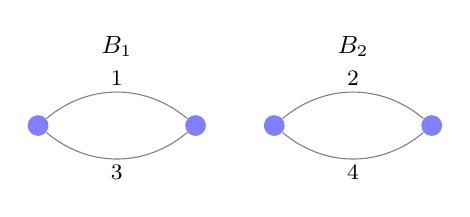
\begin{tikzpicture}[scale = 1,
%shorten >=1pt,->,
draw=black!50, node distance=\layersep]
    %\tikzstyle{every pin edge}=[<-,shorten <=1pt]
    \tikzstyle{neuron}=[circle,fill=black!25,minimum size=7.5pt,inner sep=0pt]
    \tikzstyle{output neuron}=[neuron, fill=red!50];
    \tikzstyle{n}=[neuron, fill=blue!50];

\node[n] (a) at (0,0) {};
\node[n] (b) at (2,0) {};
\node[n] (c) at (3,0) {};
\node[n] (d) at (5,0) {};
%\node[n] (e) at (6,0) {};
%\node[n] (f) at (8,0) {};
%\node at (5.5,0) {$\ldots$};
\node at (1,1) {\small $B_1$};
\node at (4,1) {\small $B_2$};
\foreach \y in {-40,40}{
%\foreach \y in {-40,0,40}{
%\draw (a) edge[bend right] node[below] {\small $2$} (b);
%\draw (a) edge[bend left] node[above] {\small $x$} (b);
\draw  (a) edge[bend left=\y] node[above] {} (b);
\draw (c) edge[bend left=\y] node[above] {} (d);
%\draw (e) edge[bend left=\y] node[above] {} (f);
};
\node at (1,0.6) {\footnotesize 1};
\node at (1,-0.6) {\footnotesize 3};
\node at (4,0.6) {\footnotesize 2};
\node at (4,-0.6) {\footnotesize 4};
\end{tikzpicture}
%
}{%
% \caption{A network for a $2 \times 2$ partnership game.}%
}
\capbtabbox{%
\footnotesize
\renewcommand{\arraystretch}{1.5}
    \centering
    \begin{tabular}{cc|c|c|}
      & \multicolumn{1}{c}{} & \multicolumn{2}{c}{P$2$}\\
      & \multicolumn{1}{c}{} & \multicolumn{1}{c}{$B_1$}  & \multicolumn{1}{c}{$B_2$} \\\cline{3-4}
      \multirow{2}*{P$1$}  & $A_1$ & $1,1$ & $2,2$ \\\cline{3-4}
      & $A_2$ & $3,3$ & $4,4$ \\\cline{3-4}
    \end{tabular}
}{%
 % \caption{\footnotesize A $2\times 2$ partnership game}%
}
\end{floatrow}
%\caption{A congestion network corresponding to a partnership game.}
\end{figure}

The congestion game to consider is shown above and a strategy of P1 is the upper or lower edges of the networks; we shall let $A_1$ be the upper edges. A strategy of P2  is the choice of a disjoint network, here the left network is P2's strategy $B_1$. For  $1\leq i \leq n$ and  $1\leq j \leq m$, where $n$ and $m$ are the number of strategies for P1 and P2 respectively, $e_{ij}$ is the $i$th edge of the $j$th disjoint network.
%We shall denote an edge in the network as $e_{ij}$, where $1\leq i \leq n$ is the edge chosen in a network and $1 \leq j\leq m$ where $n$ and $m$ are the number of strategies for P1 and P2 respectively is a chosen network.
Hence the tuple of bijective functions from the strategies of the network to the strategies in the partnership game for the congestion game shown above is:
\begin{alignat*}{4}
f_1(A_i,B_j)&=\{e_{i,j}\}_{1\leq j\leq m}, &\quad&\text{the $i$th edge in every disjoint network }\\
f_2(A_i,B_j)&=\{e_{i,j}\}_{1\leq i\leq n}, &\quad &\text{all the edges in the $j$th disjoint network}\\
\end{alignat*}
which says that every strategy in the congestion game is a subset of edges in the family of disjoint networks. The cost function $c^1_k$ for the partnership game $G^1$ is shown in the table above and the cost function for the congestion game $c_k^2(\{e_{pj}\}_{1\leq j \leq m},\{e_{iq}\}_{1\leq i \leq n})$ is the cost of the unique edge found from the intersection $\{e_{pj}\}_{1\leq j \leq m}\cap\{e_{iq}\}_{1\leq i \leq n}$.

 
\begin{figure}
\centering
\def\layersep{1.5cm}

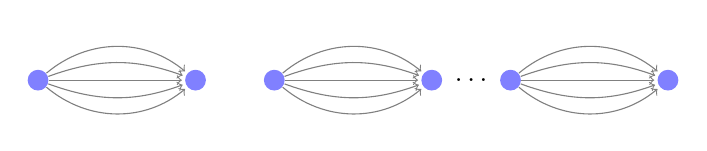
\begin{tikzpicture}[scale = 1,shorten >=1pt,->,draw=black!50, node distance=\layersep]
    \tikzstyle{every pin edge}=[<-,shorten <=1pt]
    \tikzstyle{neuron}=[circle,fill=black!25,minimum size=7.5pt,inner sep=0pt]
    \tikzstyle{output neuron}=[neuron, fill=red!50];
    \tikzstyle{n}=[neuron, fill=blue!50];

\node[n] (a) at (0,0) {};
\node[n] (b) at (2,0) {};
\node[n] (c) at (3,0) {};
\node[n] (d) at (5,0) {};
\node[n] (e) at (6,0) {};
\node[n] (f) at (8,0) {};
\node at (5.5,0) {$\ldots$};
\foreach \y in {-40,-20,0,20,40}{
%\foreach \y in {-40,0,40}{
%\draw (a) edge[bend right] node[below] {\small $2$} (b);
%\draw (a) edge[bend left] node[above] {\small $x$} (b);
\draw  (a) edge[bend left=\y] node[above] {} (b);
\draw (c) edge[bend left=\y] node[above] {} (d);
\draw (e) edge[bend left=\y] node[above] {} (f);
};
\end{tikzpicture}
\caption{A two player game with where each player has $n,m$ strategies respectively. }
\end{figure}

\begin{table}[h]
\footnotesize
\renewcommand{\arraystretch}{1.75}
    \centering
    \begin{tabular}{cc|c|c|}
      & \multicolumn{1}{c}{} & \multicolumn{2}{c}{Player $2$}\\
      & \multicolumn{1}{c}{} & \multicolumn{1}{c}{$A$}  & \multicolumn{1}{c}{$B$} \\\cline{3-4}
      \multirow{2}*{Player $1$}  & $A$ & $1,1$ & $2,2$ \\\cline{3-4}
      & $B$ & $3,3$ & $4,4$ \\\cline{3-4}
    \end{tabular}
    \caption{Partnership games}
\end{table}



\end{enumerate}


\item
\begin{enumerate}[(a)]
\item We consider two networks $A, B$ that resemble $n-$gons where $n$ is even, i.e. there are $n$ edges and $n$ vertices for each network as shown in Figure \ref{fig:ngon}. The strategy of each player $i$ is 
\begin{align*}
S_i=\{\{a_i,b_i\},\{a_{i+1},b_{i-1},b_{i+1}\}\}=\{s_i^1,s_i^2\}
\end{align*}
where $a_i,b_i$ denotes edges in $A$ and $B$ respectively and the cost function of each edge is simply $c_e(x)=x$. We claim that when all the player were to play $s_i^1$ it is a Nash equilibrium and we have the optimal value of potential which has value $2n$, since every edge is inhabit by a single player. Any player $i$ that deviates from playing $s_i^1$ will increase the potential by 2+2+2-1 (hence the claim it is a Nash) since it will share an edge with player $i+1$ in $A$ and players $i-1, i+1$ in $B$ and hence increase the potential. If all the players were to play $s_i^2$, we see that the potential will be $n+n+2n$ where the first $n$ is incurred from $A$ and the next two terms are from $B$ as we sum up the cost from 1 to the load of the edge. It is easy to see that everyone playing $s_i^2$ is a Nash; for any player that deviates from $s_i^2$, will have an increased cost of $+1$ coming from $A$, an increased cost of $+2$ from $B$ and hence this completes the proof. 



\newdimen\R
\R=2cm
\begin{figure}[h]
\centering
\begin{tikzpicture}
\tikzstyle{neuron}=[circle,fill=black!25,minimum size=5pt,inner sep=0pt]
    \tikzstyle{m}=[neuron, fill=red!50];
    \tikzstyle{n}=[neuron, fill=blue!50];

 \draw[xshift=-3cm] (-144:\R) \foreach \x in {-108,-72,...,215} {
              node[n]{}  -- (\x:\R)   
            };%--  (90:\R) ;%node[above] {t} ;%cycle (90:\R) node[above] {t} ;
\node[xshift=-6cm,below=2pt] at (-36:2.25){\footnotesize $a_{i-1}$};
\node[xshift=-6cm,below=2pt] at (-30:3.5){\footnotesize $a_i$};
\node[xshift=-6cm,below=2pt] at (-18:4.5){\footnotesize $a_{i+1}$};            
            
 \draw[xshift=3cm] (-144:\R) \foreach \x in {-108,-72,...,215} {
              node[m]{}  -- (\x:\R)   
            };
\node[below=2pt] at (-36:2.25){\footnotesize $b_{i-1}$};
\node[below=2pt] at (-30:3.5){\footnotesize $b_i$};
\node[below=2pt] at (-18:4.5){\footnotesize $b_{i+1}$};
%             \draw[xshift=3cm] (0:\R) \foreach \x in {36,72,...,359} {
%              node[m]{}  -- (\x:\R) 
%            } -- cycle (90:\R) node[above] {} ;
\end{tikzpicture}
\caption{Example with price of potential anarchy equals 2.}\label{fig:ngon}
\end{figure}

\item


%\newdimen\R
%\R=2cm
%\begin{figure}[h]
%\centering
%\begin{tikzpicture}[scale=1.5]
%\tikzstyle{neuron}=[circle,fill=black!25,minimum size=15pt,inner sep=0pt]
%    \tikzstyle{m}=[neuron, fill=red!50];
%    \tikzstyle{n}=[neuron, fill=blue!50];
%
% \draw[rotate=90,color=white] (0:\R) \foreach \x in {1,2,3} {
%              node[n](\x){\color{white}{\x}}  -- (\x*120:\R)   
%            };%--  (90:\R) ;%node[above] {t} ;%cycle (90:\R) node[above] {t} ;
%%\node[xshift=-6cm,below=2pt] at (-36:2.25){\footnotesize $a_{i-1}$};
%%\node[xshift=-6cm,below=2pt] at (-30:3.5){\footnotesize $a_i$};
%%\node[xshift=-6cm,below=2pt] at (-18:4.5){\footnotesize $a_{i+1}$};            
%\node[n](c) at (0:0){\color{white}{4}};   
%\draw[->,thick]  (1) -- (c);       
%\draw[->,thick]  (3) -- (c);       
%\draw[->,thick]  (2) -- (c);       
%\draw[->,thick] (1) -- (2);
%\draw[->,thick] (2) -- (3);
%\draw[->,thick] (3) -- (1);
%% \draw[xshift=3cm] (-144:\R) \foreach \x in {-108,-72,...,215} {
%%              node[m]{}  -- (\x:\R)   
%%            };
%%\node[below=2pt] at (-36:2.25){\footnotesize $b_{i-1}$};
%%\node[below=2pt] at (-30:3.5){\footnotesize $b_i$};
%%\node[below=2pt] at (-18:4.5){\footnotesize $b_{i+1}$};
%%             \draw[xshift=3cm] (0:\R) \foreach \x in {36,72,...,359} {
%%              node[m]{}  -- (\x:\R) 
%%            } -- cycle (90:\R) node[above] {} ;
%\end{tikzpicture}
%\caption{Example with price of potential anarchy equals 2.}\label{fig:3gon}
%\end{figure}



 
\end{enumerate}

\end{enumerate}











\end{document}